\documentclass[a4paper, 11pt]{article}
\usepackage{graphicx}
\usepackage[a4paper,bindingoffset=0in,%
            left=1in,right=1in,top=1in,bottom=1in,%
            footskip=.25in]{geometry}
\usepackage[square, numbers]{natbib}
\usepackage{amsmath}
\usepackage{amssymb}
\usepackage{mathtools}
\usepackage{algorithm}
\usepackage{algorithmic}
\newcommand{\Data}{\mathcal{D}}
\newcommand{\Node}{\mathcal{N}}
\newcommand{\Split}{\mathcal{S}}

\begin{document}

\title{A Software Package for Extendable Decision Trees in C++}

\begin{titlepage}
	\centering
	\vspace{1cm}
	{\scshape\LARGE Ludwig-Maximilians-Universität München \par}
	\vspace{1.5cm}
	
\includegraphics[width=0.35\textwidth]{figure/lmu_logo.png}\par\vspace{1cm}
	\vspace{0.5cm}
	{\scshape\Large Bachelor Thesis in Computer Science\par}
	\vspace{1.5cm}
	{\huge\bfseries treelib - A Software Package for Extendable Decision Trees in C++\par}
	\vspace{2cm}
	{\Large\itshape Christian Alexander Scholbeck\par}
	\vfill
	supervised by\par
	Prof. Dr. Bernd Bischl \par
	Prof. Dr. Marvin Wright \par
	Dr. Giuseppe Casalicchio

	\vfill

% Bottom of the page
	{\large Month Day, 2021 \par}
\end{titlepage}

\newpage
\thispagestyle{empty}

\begin{abstract}
This thesis provides a software package for extendable decision trees written in C++. The package follows object-oriented and modular design principles. It works as a standalone application, or can be called by other programming languages. It supports both binary and multiway splitting, and can be extended with new optimizing algorithms, split criteria, models, and objectives. Supported application areas include classic predictive modeling with decision trees such as CART or C4.5, and advanced modeling such as model-based recursive partitioning. Furthermore, the modular design principle allows the extension of the package to support novel applications such as surrogate modeling for interpretable machine learning.
\end{abstract}
\vspace*{1cm}
\tableofcontents
\clearpage
\setcounter{page}{1}
\section{Introduction}

Decision trees are one of the most fundamental techniques in machine learning. They are frequently preferred over more complex models due to their intelligibility in the form of decision rules, e.g., in medical applications \cite{podgorelec_trees_medicine}. Tree learning algorithms are numerous and differ regarding split criteria, model choices, stopping rules and pruning. \par
Ideas for decision tree learning originate in supervised learning and date back as far as linear discriminant analysis \cite{fisher_lda}. A large variety of decision tree algorithms has been published, such as Automatic Interaction Detection (AID) \cite{hawkins_AID}, Theta AID (THAID) \cite{ messenger_mandell_thaid}, Chi-Squared AID (CHAID) \cite{kass_chaid}, Classification and Regression Trees (CART) \cite{cart_1, hastie_elemstatlearn}, C4.5 \cite{quinlan_c45}, and many more \cite{loh_trees_review}.
\par
So-called hybrid, model, or functional trees \cite{zeileis_mob} have added capabilities such as fitting node models \cite{quinlan_model_tree}, or using linear combinations of variables for splits \cite{brodley_multivariate_trees}. Hybrid trees are also capable of unsupervised learning, e.g., by training kernel density estimators inside the nodes \cite{ram_density_estimation_tree}.
Recent developments have embedded hybrid trees into frameworks for  statistical inference, e.g., conditional inference trees \cite{hothorn_ctree} and model-based recursive partitioning (MOB) \cite{zeileis_mob}.
\par
A critical drawback of decision trees is a high variance under perturbations of the training data \cite{hastie_elemstatlearn}. This has led to the development of tree ensembles such as random forests \cite{breiman_randomforests}, which reduce variance to the detriment of losing interpretability.

%Popular variants include classification and regression trees (CART) \cite{cart_1}, C4.5 \cite{quinlan_c45}, and model-based recursive partitioning \cite{zeileis_mob}.
\par
%Their most critical drawback is a high variance under perturbations of the training data \cite{hastie_elemstatlearn}. This has led to the development of tree ensembles such as random forests \cite{breiman_randomforests}, which reduce variance to the detriment of losing interpretability.

%such as CART minimize the sum of squared deviations from the mean target value for regression tasks, or Gini impurity for classification tasks. More complex variants such as MOB train predictive models inside the leaf nodes, e.g., (generalized) linear models. Most decision tree variants such as CART or MOB are restricted to binary splits, whereas others such as C4.5 enable multiway splitting, which increases computational complexity.
%\par
%The possibilities of applying decision trees in contexts other than such as interpretable machine learning are numerous. For instance, due to their intelligibility, decision trees are especially suited as a surrogate model for black box models, where the black box predictions are approximated by interpretable functions inside the leaf nodes.
\par
Applications for decision trees are diverse, e.g., predictive modeling \cite{hastie_elemstatlearn}, surrogate modeling \cite{schaaf_surrogate_tree}, or density estimation \cite{ram_density_estimation_tree}. This creates a requirement for an accessible, efficient, and extendable software implementation of decision trees. Accessible, to benefit a broad scientific community. Efficient, as the computational demand of optimizing splits grows considerably with the tree's complexity. Extendable, as different applications require different decision tree setups.
\par

\subsection{Contributions and Structure} The central contribution of this thesis is a from-the-ground-up implementation of extendable decision trees as an open-source software package. The package is written in \texttt{C++} to achieve a high degree of computational efficiency, while preserving object-oriented principles and portability to other programming languages. The package follows modular design principles to achieve a maximum degree of extensibility.
\par
The written thesis provides a short theoretical overview on decision trees, describes the software design and extensibility, and demonstrates the package on simulated and real data. Over the years, the number of published decision tree algorithms has grown tremendously. The purpose of the theoretical section is not to provide an exhaustive review of available techniques, which would go beyond the scope of a thesis. Instead, it shall provide a compact introduction to the topic and pave the way for the description and demonstration of the software package.

\subsection{Software Description}

The software can be run as a standalone application, and supports console outputs of tree information such as the tree structure, and node summaries. Furthermore, it can be called by other programming languages for the usage in more flexible application environments. The program specifications are determined at runtime. It supports an arbitrary number of splits.
The package is equipped with two types of objective functions; sum of squared errors (SSE) for regression tasks, and the Gini impurity for classification tasks. Node models include: majority vote (classification), mean target value (regression), and linear regression model (regression and classification).
The modular structure allows for the extension with 
new optimizing algorithms, split criteria, node models, and objectives. 

\section{Related Work}

An initial software implementation of MOB was published as part of the \texttt{party} package \cite{party_package} for the \texttt{R} programming languge for statistical computing \cite{r_citation}. A more flexible version, which supports more inference options and is extendable to new models, was introduced in the \texttt{partykit} package \cite{partykit_package}. 
\par
The \texttt{R} language is able to directly call \texttt{C} or \texttt{C++} code, which warrants significant speedups in computational execution time \cite{eddelbuettel_rcpp}. However, software implementations which are solely written in \texttt{R} code such as \texttt{partykit} pose a considerable bottleneck in computational speed.
The software package \texttt{ranger} \cite{ranger_package} provides a fast implementation of random forests in \texttt{C++} and can be directly called from the identically named \texttt{R} package. However, it is restricted to random forests and intextendable regression trees.

\section{Theory}

A decision tree is a hierarchical structure based on recursive partitioning of the data. Each partitioning of the data is referred to as a node, whereas a final partitioning is referred to as a leaf node.
The starting point of a decision tree, which encompasses the entire, unpartitioned data, corresponds to the root node. Nodes excluding leaf nodes and root node are also referred to as internal nodes.
A split node becomes a parent node, and the resulting nodes become children or child nodes. Subsequent partitionings can be visualized as a series of decision rules, which together form a tree graph (see Fig. \ref{fig:tree_structure}). Decision trees are $k$-ary if each node has $k$ children.
Binary trees with $k = 2$ are the most popular variant \cite{hastie_elemstatlearn}. Furthermore, there are trees with varying numbers of child nodes \cite{quinlan_c45}. Decision trees are often termed according to their application area, e.g., regression \cite{cart_1}, classification \cite{quinlan_c45, cart_1, kass_chaid}, survival \cite{derose_survival_tree}, or density estimation trees \cite{ram_density_estimation_tree}.

\begin{figure}
    \centering
    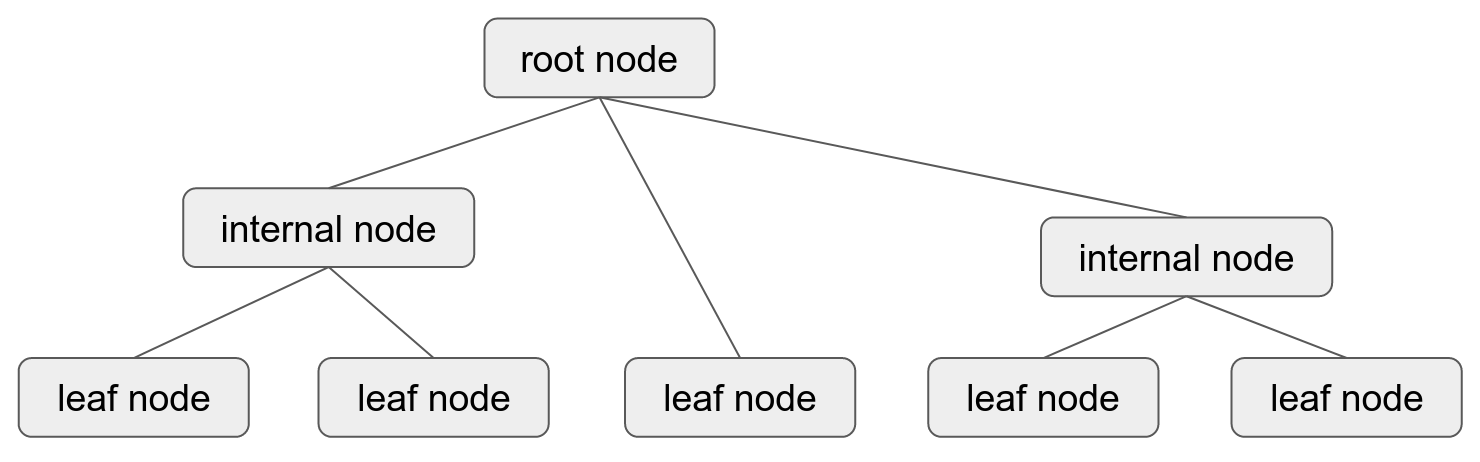
\includegraphics[width = 0.6 \linewidth]{thesis/figure/decision_tree_structure.png}
    \caption{General decision tree structure comprising a root node, regular nodes, and leaf nodes.}
    \label{fig:tree_structure}
\end{figure}

\subsection{Notation}

We consider a $p$-dimensional feature space $\mathcal{X} = \mathcal{X}_1 \times \dots \times \mathcal{X}_p$ and a target space $\mathcal{Y}$. The probability distribution $\mathcal{P}$ is defined on the sample space $\mathcal{X}_p \times \mathcal{Y}$. A decision tree is trained on a data set $\mathcal{D}$ that was drawn from $\mathcal{P}$ with a prediction function $\widehat{f}: \mathbb{R}^p \mapsto \mathbb{R}^g$ with $g \in \mathbb{N}$. An observation or instance is denoted by $x = (x_1, \dots, x_p)$. The value of the $j$-th feature in $x$ is denoted by $x_j$. The target vector is denoted by $y$. The 
$i$-th observation and target value in $\Data$ are denoted by $x^{(i)}$ and $y^{(i)}$, respectively. $\Data$ corresponds to the root node. A split $\Split$ partitions a node $\Node$ into multiple 
children $\{\Node_1, \dots, \Node_k\}$, which correspond to mutually exclusive subspaces of $\Node$.  For binary splits, the child nodes $\Node_1$ and $\Node_2$ correspond to half-planes. The split is evaluated by an objective function $Obj(\Node, \Split)$.
A continuous split corresponds to a variable $x_j$ and one or multiple thresholds. The threshold can be a scalar or an interval. A categorical split is based on one or multiple feature categories according to which the data is partitioned.


% Given a single node $R$, a splitting feature $j$ and a split point $q$, we define the pair of half-planes $R_1(j, q) = \{x \;\vert\; x_j \leq q\}$ and $R_2(j, q) = \{x \;\vert\; x_j > q\}$ with the respective cAME values $\text{cAME}_1 = \frac{1}{n} \sum_{i \;:\; x^{(i)} \;\in\; R_1(j, q)} \text{fME}_S(x^{(i)}, h_S)$ and $\text{cAME}_2 = \frac{1}{n} \sum_{i \;:\; x^{(i)} \;\in\; R_2(j, q)} \text{fME}_S(x^{(i)}, h_S)$. The goal is to find the pair $(j, q)$ that solve the following minimization problem:

%\par
%Training more complex models inside the nodes such as (generalized) linear models increases the predictive performance of the decision tree, but increases computational costs. Training a complex model for every potential split is infeasible in practice. 


% \subsection{General Setup}

% Each decision tree has five common components:
% \begin{enumerate}
%     \item \textbf{Node model choice:} A node model can be of any type.
    
%     e.g., none (if the objective does not require predictions), a constant, a (generalized) linear model, or a kernel density estimate. The model type can vary across nodes.
%     \item \textbf{Objective function:} 
%     The objective function determines the selection of a split. Its characteristics depend on the purpose of the decision tree, e.g., the L2 loss for predictive modeling, or the integrated squared error for kernel density estimation \cite{ram_density_estimation_tree}. The objective may vary across nodes, e.g., computational costs can be decreased by using a heuristic for initial splits with many observations. 
%     \item \textbf{Optimization:} For each node, we need to find one or multiple split points that improve the objective given certain hyperparameters such as the minimum node size.
%     \item \textbf{Stopping:} We may either split the tree down as far as possible, or use an early stopping criterion.
%     \item \textbf{Pruning:} To avoid overfitting, the tree can be pruned post-hoc.
% \end{enumerate}

\subsection{Methodological Overview}

Growing a tree by global optimization poses considerable computational difficulties \cite{norouzi_nongreedy_tree}. Thereby, the default approach is through greedy optimization of an objective function. A tree can be grown via batch processing, i.e., the entire training data is available at once, or incrementally, e.g., for data streams \cite{potts_incremental_model_tree}. Pruning weighs the trade-off between growing a tree too large and too small \cite{hastie_elemstatlearn}. A tree with too many splits generally results in a smaller training error and a larger generalization error (overfitting). Conversely, a tree with few splits both performs bad on test, as well as on training data (underfitting). There are two options to prune a tree: pre- and post-pruning. Pre-pruning incorporates an early stopping criterion, while post-pruning fully grows the tree and removes nodes post-hoc. Post-pruning methods can further be classified as top-down, e.g., pessimistic error pruning \cite{quinlan_simplifying}, or bottom-up, e.g., reduced error pruning \cite{quinlan_simplifying}.
\par
A greedy algorithm iteratively partitions a node, and compares the objective computed on the parent, and on the children. The objective for all children is aggregated, e.g., averaged, summed up, or weighted by the fraction of node observations before being summed up. The algorithm then chooses the split with the maximum improvement in objective value. Through recursion, this procedure is repeated for each node.

\par 
One simple option is to reduce the impurity of target values inside each node. CART aims to reduce impurity by minimizing the total sum of squares (TSS), which is proportional to the sample variance (for regression tasks) and Gini impurity for classification tasks:
\begin{align}
TSS(\Node) &= \sum_{i \;:\; (x, y)^{(i)} \;\in\; \Node} \left(y^{(i)} - \overline{y}\right)^2
\label{eq:cart_regr}
\end{align}
Consider a node with $n$ observations. The frequencies of all target categories $1, \dots, k$ correspond to $n_1, \dots, n_k$. The Gini coefficient is defined as:
$$
Gini(\Node) = 1 - \sum_{i = 1}^n \left(\frac{n_i}{n}\right)^2
$$
CART has proven to provide a fairly good predictive performance compared to more complex models such as neural networks \cite{razi_cart_comparison}, while being much less complex.
\par
Model trees aim to boost predictive performance while preserving the decision tree's intelligibility by training leaf node models. In fact, Eq. (\ref{eq:cart_regr}) already implicitly incorporates a simple leaf node model: the target average. The model can be made explicit by rewriting each TSS as the sum of squared errors (SSE) between target values and the model prediction, also referred to as the residual sum of squares:
\begin{align*}
SSE(\Node) = \sum_{i \;:\; (x, y)^{(i)} \;\in\; \Node} \left(y^{(i)} - \widehat{f}(x^{(i)})\right)^2
\end{align*}
\par
The algorithm M5 \cite{quinlan_model_tree} is an extension of ordinary decision trees that trains linear regression models inside the leafs. It starts with growing a decision tree by minimizing the target standard deviation inside each node. It then punes the tree, and adds linear regression models to the leafs. M5' \cite{wang_m5} is a modification of M5, e.g., regarding the handling of missing values.
\par
Training linear leaf node models (via least squares), whereas the splits have been determined via minimization of the target standard deviation, results in suboptimal leaf node models. Instead, a more favorable approach is to use the same objective for both model estimation and splitting \cite{zeileis_mob}. The RETIS algorithm \cite{karalic_retis} minimizes the sum of child node SSE values. For each evaluated split, this requires the calculation of a least squares estimate for all models which quickly becomes infeasible in practice. Computational costs can be decreased by reducing the model complexity, e.g., by restricting the number of explanatory variables \cite{grimshaw_treed}, which limits predictive performance. In \cite{potts_incremental_model_tree} linear leaf node models are estimated incrementally through each split. The authors argue that splitting a node and estimating multiple linear models always provides a better or equal SSE compared to a single linear model.
Instead, the authors propose a statistical test based on the Chow test \cite{chow_inequality_test}. Furthermore, there is a large variety of techniques that support more complex models such as generalized linear models \cite{ciampi_glm_tree, loh_guide, gama_functional_tree, zeileis_mob}. For instance, MOB provides a framework for a multitude of parametric node models, where the splits are found through a model-specific parameter instability test.

\subsection{Binary versus Multiway Splits}

Most techniques such as CART create binary decision trees. A series of binary splits is able to represent the same data partitioning as a multiway split, while the latter also creates more fragmented trees  \cite{hastie_elemstatlearn} (see Fig. \ref{fig:binary_vs_multiway}). On the other hand, a multiway split is easier comprehensible to the human mind, which is not used to think of decisions with multiple outcomes as a series of decisions with binary outcomes. Furthermore, greedy optimization is not guaranteed to find the same series of binary decisions as an algorithm that considers multiway decisions. Greedy optimization makes decision trees subject to a high variance, as a decision higher up cascades through the entire tree and results in different splits lower down the tree \cite{hastie_elemstatlearn}.
\begin{figure}
    \centering
    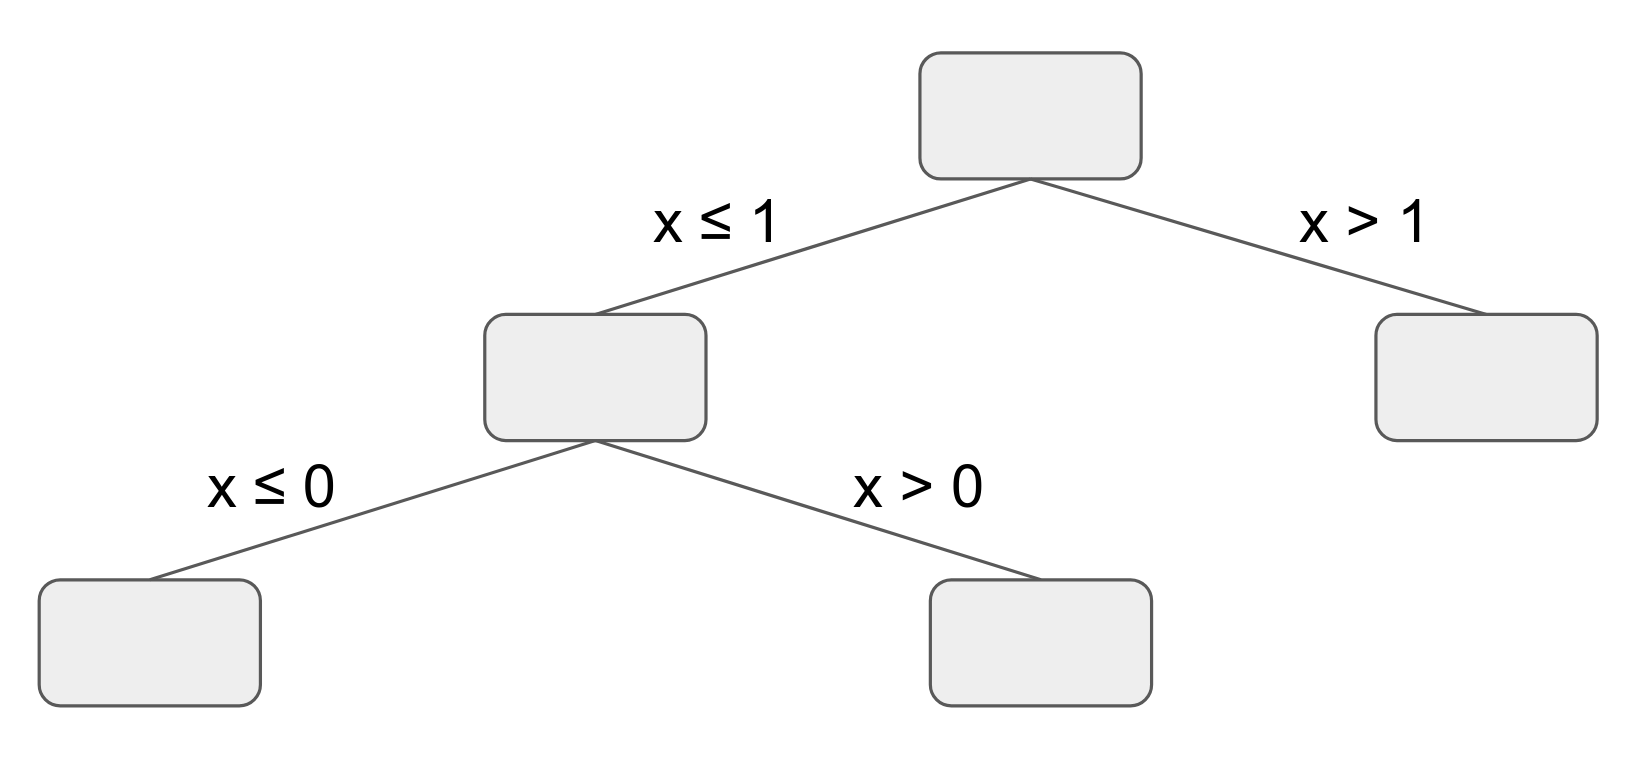
\includegraphics[width = 0.59\linewidth]{thesis/figure/binary_splits.png}
    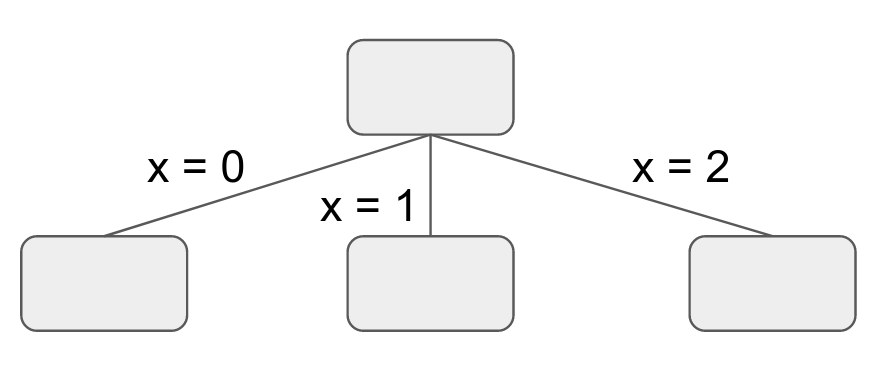
\includegraphics[width = 0.4\linewidth]{thesis/figure/threeway_split.png}
    \caption{A binary decision tree (left) is able to represent the same partitioning as the multiway split.}
    \label{fig:binary_vs_multiway}
\end{figure}
\par
When allowing for multiway splits, one needs to decide whether to train a $k$-ary tree, i.e., each node has $k$ children, or the number of children is chosen adaptively. The latter creates two predicaments. First, the objective function cannot be updated from one split to the next, thereby considerably increasing computational costs (see Section \ref{sec:computational_speedups}). Second, we need to construct an algorithm that decides how many children to create. If the objective is based on the aggregated model fit of all child nodes, we can expect more splits to always provide a better fit. Multiway splitting therefore boils down to a regularization problem.

\section{Computational Speedups}
\label{sec:computational_speedups}

With a growing complexity, e.g., due to the cost of training node models for every split or multiway splitting, the computational cost of decision trees grows considerably. This puts a great importance on an efficient split search, which can be achieved in multiple ways.
First, computations can be parallelized, e.g., after splitting a node, the computations in all child nodes are independent of each other and can run in parallel.
Second, we can evaluate a subset of values, e.g., if the split variable is continuous, close values can be omitted from the search.
Third, for each node there is a large number of split points to be evaluated. Instead of recomputing the objective and model for each split from scratch, computations may be sped up by an update mechanism. Fourth, a split point generator can suggest split points with a higher probability of improving the objective than other points.

\subsection{Updating Objective Functions}

Updating an objective function is restricted to $k$-ary trees, as we have to update the same node in each iteration. Consider two splits $S_A$ and $S_B$, which result in different child nodes (but with the same index) $N_1$ and $\tilde{N}_1$. An update mechanism decomposes the objective function $Obj(N, S_B)$ such that it depends on $Obj(N, S_A)$, as well as on additional observations $\mathcal{N}_1 \setminus \mathcal{N}_0$, and missing ones $\mathcal{N}_0 \setminus \mathcal{N}_1$. 

\subsubsection{Mean Prediction}

The mean prediction is updated by keeping tack of the cumulative sum of target values. Let $\overline{y}_0$ the initial target mean value:
$$
\overline{y}_0 = \frac{1}{n_0} \sum_{i = 1}^n y^{(i)} = \frac{1}{n_0} M
$$
The updated target mean corresponds to:
$$
\overline{y}_1 =  \frac{1}{n_0 + \vert \mathcal{D}_1 \setminus \mathcal{D}_0 \vert - \vert \mathcal{D}_0 \setminus \mathcal{D}_1 \vert}\left(M + \sum_{i \,:\, x^{(i)} \, \in \, \mathcal{D}_1 \setminus \mathcal{D}_0} y^{(i)} - \sum_{i \,:\, x^{(i)} \, \in \, \_0 \setminus \mathcal{D}_1} y^{(i)} \right)
$$

\subsubsection{Linear Regression Models}

Given a set of training observations X and the target vector Y, the coefficients of a  linear regression model are estimated by:
\begin{equation}
\Theta = (X^TX)^{-1}X^TY
\label{eq:linmod_beta}
\end{equation}
The model prediction is given by $y = x^T \Theta$. The residual between observed target value and model prediction is given by the squared error $\epsilon = (y - \hat{y})^2 = (y - x^T \Theta)^2$. Eq. (\ref{eq:linmod_beta}) can be recursively estimated for a series of observations \cite{potts_incremental_model_tree}:
% \begin{align*}
%     \Theta_i &= \Theta_{i - 1} + \frac{(X^TX)^{-1}_{i-1} \, x_i \left(y_i - x_i^T\Theta_{i-1}\right)}{1 + x_i^T \, (X^T X)_{i-1} \, x_i} \\
%     (X^TX)^{-1}_i &= (X^TX)^{-1}_{i-1} - \frac{(X^TX)^{-1}_{i-1} \, x_i \, x_i^T \, (X^TX)^{-1}_{i-1}}{1 + x_i^T (X^TX)^{-1}_{i-1} x_i} \\
%     \text{SSE}_i &= \text{SSE}_{i-1} + \left(y_i - x_i^T \Theta_{i-1}\right) \left(y_i - x_i^T \Theta_i\right)
% \end{align*}
\begin{align*}
    \Theta_i &= \Theta_{i - 1} + \frac{B^{-1}_{i-1} \, x_i \left(y_i - x_i^T\Theta_{i-1}\right)}{1 + x_i^T \, B_{i-1} \, x_i} \\
    B^{-1}_i &= B^{-1}_{i-1} - \frac{B^{-1}_{i-1} \, x_i \, x_i^T \, B^{-1}_{i-1}}{1 + x_i^T B^{-1}_{i-1} x_i} \\
    \text{SSE}_i &= \text{SSE}_{i-1} + \left(y_i - x_i^T \Theta_{i-1}\right) \left(y_i - x_i^T \Theta_i\right)
\end{align*}
where $B = X^TX$.
It follows that for two splits, $\Theta$ can be updated via Algorithm \ref{algo:rec_lm}:
\begin{algorithm}
 \caption{Updating Linear Regression Model \label{algo:rec_lm}}
 \begin{algorithmic}[1]
 \renewcommand{\algorithmicrequire}{\textbf{Input}: $\Theta, B, \text{SSE}, \mathcal{D}_0, \mathcal{D}_1$}
 \renewcommand{\algorithmicensure}{\textbf{Output}: $\Theta_{updated}, \text{B}_{updated}, \text{SSE}_{updated}$}
 \REQUIRE
 \ENSURE
 \FORALL{$(x^{(i)} \in \mathcal{D}_0 \setminus \mathcal{D}_1)$}
    \STATE
    $\Theta_{temp} = \Theta$
    \STATE
    $\Theta = \Theta - \frac{B^{-1}_{i-1} \, x_i \left(y_i - x_i^T\Theta\right)}{1 + x_i^T \, B_{i-1} \, x_i}$
    \STATE
    $B^{-1} = B^{-1} - \frac{B^{-1} \, x_i \, x_i^T \, B^{-1}}{1 + x_i^T B^{-1} x_i}$
    \STATE
    $\text{SSE} = \text{SSE} - \left(y_i - x_i^T \Theta\right) \left(y_i - x_i^T \Theta_{temp}\right)$
 \ENDFOR 
 \FORALL{$(x^{(i)} \in \mathcal{D}_1 \setminus \mathcal{D}_0)$}
    \STATE
    $\Theta_{temp} = \Theta$
    \STATE
    $\Theta = \Theta + \frac{B^{-1}_{i-1} \, x_i \left(y_i - x_i^T\Theta\right)}{1 + x_i^T \, B_{i-1} \, x_i}$
    \STATE
    $B^{-1} = B^{-1} + \frac{B^{-1} \, x_i \, x_i^T \, B^{-1}}{1 + x_i^T B^{-1} x_i}$
    \STATE
    $\text{SSE} = \text{SSE} + \left(y_i - x_i^T \Theta_{temp}\right) \left(y_i - x_i^T \Theta\right)$
 \ENDFOR
 \RETURN $\Theta, B, \text{SSE}$;
 \end{algorithmic} 
\end{algorithm}
\subsection{Updating Objective Functions}

Consider two sets of observations $\mathcal{D}_0$ and $\mathcal{D}_1$. An update mechanism decomposes the objective function $O(\mathcal{D})$ such that $O(\mathcal{D}_1)$ depends on $O(\mathcal{D}_0)$, as well as on additional observations $\mathcal{D}_1 \setminus \mathcal{D}_0$, and missing ones $\mathcal{D}_0 \setminus \mathcal{D}_1$. Updating an objective is only viable for a fixed number of child nodes per node, as the update rule always updates a single, fixed child node.

\subsubsection{Total Sum of Squares}

The total sum of squares (TSS) corresponds to the the sum of squared deviations between target values and the target average:
$$
\text{TSS}(y) = \sum_{i = 1}^{n} \left(y^{(i)} - \overline{y}\right)^2
$$
The TSS is used by algorithms such as CART. Averaging the TSS yields a variance estimate:
$$
\widehat{Var}(y) = \frac{1}{n-1}\, \text{TSS}(y)
$$
The TSS can be decomposed as follows:
$$
\text{TSS}(y) = \sum_{i = 1}^{n} \left(y^{(i)}\right)^2 - \overline{y}^2
$$

\subsubsection{Sum of Squared Errors}

The TSS is equivalent to the sum of squared errors (SSE), also referred to as the L2 loss, if the trained model corresponds to the mean target value:
\begin{align*}
\text{SSE}(\mathcal{D}) &= \sum_{i = 1}^{n} \left(y^{(i)} - \hat{f}\left(x^{(i)}\right)\right)^2 \\
&= \sum_{i = 1}^{n} \left[\left(y^{(i)}\right)^2 - 2\, y^{(i)} \hat{f}\left(x^{(i)}\right) + \hat{f}\left(x^{(i)}\right)^2\right] \\
&= \sum_{i = 1}^{n} \left(y^{(i)}\right)^2 - 2 \sum_{i = 1}^{n} \,y^{(i)} \hat{f}\left(x^{(i)}\right) + \sum_{i = 1}^{n} \hat{f}\left(x^{(i)}\right)^2 \\
\end{align*}
Consider two multiway splits, each one partitioning a node into $k$ subsets. We update the left-most node, which contains $n_0^{(0)}$ observations in the first split, and $n_0^{(1)}$ in the second one. The corresponding SSEs are denoted by $\text{SSE}^{(0)}$ and $\text{SSE}^{(1)}$. The child node observations resulting from each split are denoted by $\mathcal{D}_0$ and $\mathcal{D}_1$.

The SSE for the second split can be decomposed as:
\begin{align}
\text{SSE}^{(1)}\left(\mathcal{D}_0 \cup \mathcal{D}_1\right) &= \text{SSE}^{(0)}(\mathcal{D}_0) \nonumber \\
&\phantom{{}={}} + \sum_{i \,:\, x^{(i)} \, \in \, \mathcal{D}_1 \setminus \mathcal{D}_0} \left(y^{(i)}\right)^2 - 2 \sum_{i \,:\, x^{(i)} \, \in \, \mathcal{D}_1 \setminus \mathcal{D}_0} \,y^{(i)} \hat{f}\left(x^{(i)}\right) + \sum_{i \,:\, x^{(i)} \, \in \, \mathcal{D}_1 \setminus \mathcal{D}_0} \hat{f}\left(x^{(i)}\right)^2 \nonumber \\
&\phantom{{}={}} - \sum_{i \,:\, x^{(i)} \, \in \, \mathcal{D}_0 \setminus \mathcal{D}_1} \left(y^{(i)}\right)^2 + 2 \sum_{i \,:\, x^{(i)} \, \in \, \mathcal{D}_0 \setminus \mathcal{D}_1} \,y^{(i)} \hat{f}\left(x^{(i)}\right) - \sum_{i \,:\, x^{(i)} \, \in \, \mathcal{D}_0 \setminus \mathcal{D}_1} \hat{f}\left(x^{(i)}\right)^2 \label{eq:SSE_update}
\end{align}

%The child node SSEs are denoted by $SSE_1, \dots, SSE_k$. The SSE  with $n_1$ observations and target vector $y_1$ can be decomposed as:
%$$
%L_1^{(0)}(y_1) = \sum_{i = 1}^{n_1} \left(y_1^{(i)} - \overline{y_1}\right) = \sum_{i = 1}^{n_1} \left(y_1^{(i)}\right)^2 - \sum_{i = 1}^{n_1} y_1^{(i)} 
%$$

%For classification trees, CART minimizes Gini impurity, which summarizes the distribution of relative target class frequencies. 
%CART is restricted to binary splits. The tree is fully grown until a pre-specified minimum node size criterion would be violated when splitting further. The tree height is pruned post-hoc according to a complexity parameter to avoid overfitting, which is estimated via cross-validation. Missing values are handled via surrogate splits.


%\par
%C4.5 is similar to CART, but is restricted to classification trees. It uses an information-theoretic measure of node impurity called gain ratio, which corresponds to the quotient between information gain and entropy. C4.5 conducts multiway splits for categorical variables, i.e., all observations of the same category are binned together. Additional differences between CART and C4.5 can be found for missing values, which requires surrogate splitting.
%\par
%Consider a binary split which partitions a node into two subsets with $n_1$ and $n_2$ observations, and child node TSS $L_1$ and $L_2$. The left node TSS with $n_1$ observations and target vector $y_1$ can be decomposed as:
%$$
%L_1^{(0)}(y_1) = \sum_{i = 1}^{n_1} \left(y_1^{(i)} - \overline{y_1}\right) = \sum_{i = 1}^{n_1} \left(y_1^{(i)}\right)^2 - \sum_{i = 1}^{n_1} y_1^{(i)} 
%$$
%For the next split value, there are two different partitionings with either $n_1 + 1$ and $n_2 - 1$, or $n_1 - 1$ and $n_2 + 1$ observations. For the first option, the loss can be updated as:
%$$
%L_1^{(1)}(y_1) = L_1^{(0)} + y_{1}^{(n_1 + 1)} - y_{1}^{(n_1 + 1)}
%$$
%For the second option, it can be updated as:
%$$
%L_1^{(1)}(y_1) = L_1^{(0)} - y_{1}^{(n_1)} + y_{1}^{(n_1)}
%$$



\subsection{Split Point Generation}




\section{Software Design}

\section{Extensibility}

\section{Demonstrations and Benchmarks}

\section{Conclusion}
\bibliographystyle{plainnat}
\bibliography{bibfile}


\end{document}